\documentclass{article}

% Language setting
% Replace `english' with e.g. `spanish' to change the document language
\usepackage[english]{babel}

% Set page size and margins
% Replace `letterpaper' with `a4paper' for UK/EU standard size
\usepackage[letterpaper,top=2cm,bottom=2cm,left=3cm,right=3cm,marginparwidth=1.75cm]{geometry}

% Useful packages
\usepackage{enumerate}
\usepackage[shortlabels]{enumitem}
\usepackage{amsmath, amsfonts, amssymb, mathtools}
\usepackage{graphicx}
\usepackage[colorlinks=true, allcolors=blue]{hyperref}
\usepackage[table]{xcolor}  % For coloring rows
\usepackage{ tipa }
\usepackage[section]{placeins}
\usepackage{float} % For 'H' option of images

% For drawing state machine
\usepackage{tikz}
\usetikzlibrary{automata} % Import library for drawing automata
\usetikzlibrary{positioning} % ...positioning nodes
\usetikzlibrary{arrows} % ...customizing arrows
\tikzset{
    node distance=3cm, % Minimum distance between two nodes. Change if necessary.
    every state/.style={ % Sets the properties for each state
        thick,
        fill=gray!10
    },
    initial text={}, % No label on start arrow
    double distance=2pt, % Adjust appearance of accept states
    bend angle=15,
    every edge/.style={ % Sets the properties for each transition
        draw,
        ->,>=stealth, % Makes edges directed with bold arrowheads
        auto,
        thick
    }
}
            
\let\epsilon\varepsilon

\newcommand{\N}{\mathbb{N}}

\title{
Cyber Physical Systems - Discrete Models \\
[0.2em]Exercise Sheet 5 Solution
}
\author{
  Alper Ari\\
  \texttt{aa508@uni-freiburg.edu}
  \and
  Onur Sahin\\
  \texttt{os141@uni-freiburg.de}
}
\date{\today}

\begin{document}
\maketitle

\section*{Exercise 1: Synchronization}
Given two transition systems $T = (S, Act, \longrightarrow, S_0, AP, L)$ and $T_0' = (S', Act', \longrightarrow ', S_0, AP', L')$ \\

\begin{enumerate}[(a)]
     \item{Give a set Syn such that $T||T'$ and $T ||_{Syn} T'$ are always equivalent:} $Syn = Act \cap Act'$
     \item{Give a set Syn such that $T|||T'$ and $T ||_{Syn} T'$ are always equivalent:} $Syn = \emptyset$
\end{enumerate}


\section*{Exercise 2: Coffee Machine and Transition System}
\begin{enumerate}[(a)]
    \item{Transition system of corresponding program graph}
    \begin{figure}[H]
        \centering
        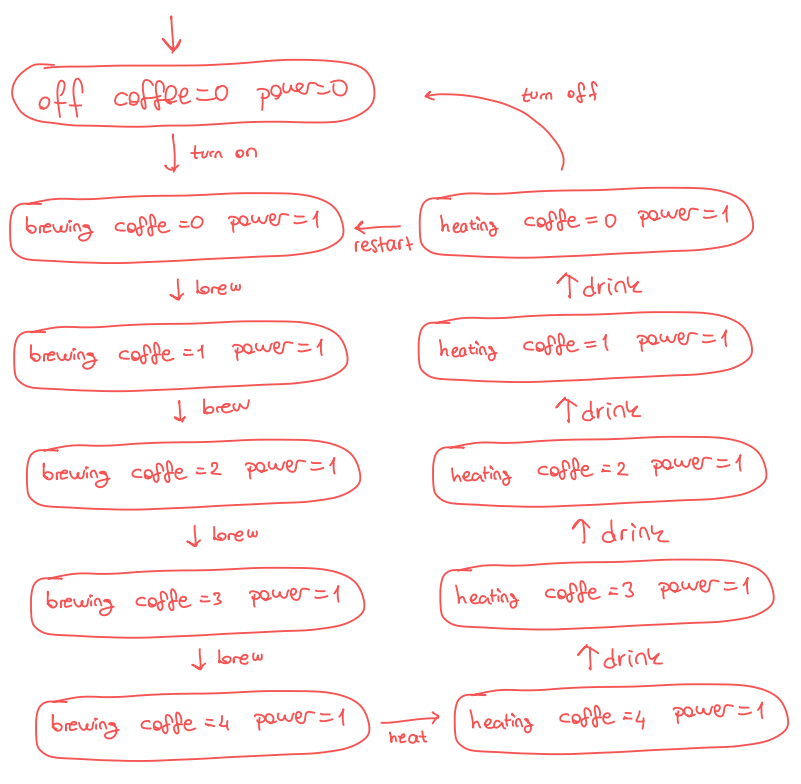
\includegraphics[width=4in]{images/2a.png}
        \caption{Transition system of coffee machine}
        \label{fig:2a}
    \end{figure}
    And some example transitions whose existence can be justified by SOS rule:
    \begin{enumerate}[i]
        \item \texttt{Transition 1:}
        $$\frac{
            \text{brewing}\xrightarrow{\text{coffee}<4:\text{brew}} \text{brewing}  \wedge \{\text{coffee}=0, \text{power}=1\} \models (\text{coffee}<4)
        }{
            \langle \text{brewing}, \{\text{coffee}=0, \text{power=1}\} \rangle 
            \xrightarrow{\text{brew}}
            \langle \text{brewing}, \{\text{coffee}=1, \text{power=1}\} \rangle 
        }$$\\
        
        \item \texttt{Transition 2:}
        $$\frac{
            \text{heating}\xrightarrow{\text{coffee}>0:\text{drink}} \text{heating}  \wedge \{\text{coffee}=4, \text{power}=1\} \models (\text{coffee}>0)
        }{
            \langle \text{heating}, \{\text{coffee}=4, \text{power=1}\} \rangle 
            \xrightarrow{\text{drink}}
            \langle \text{heating}, \{\text{coffee}=3, \text{power=1}\} \rangle 
        }$$\\
        
        \item \texttt{Transition 3:}
        $$\frac{
            \text{brewing}\xrightarrow{\text{coffee}=4:\text{heat}} \text{heating}  \wedge \{\text{coffee}=4, \text{power}=1\} \models (\text{coffee}=4)
        }{
            \langle \text{brewing}, \{\text{coffee}=4, \text{power=1}\} \rangle 
            \xrightarrow{\text{heat}}
            \langle \text{heating}, \{\text{coffee}=4, \text{power=1}\} \rangle 
        }$$\\
    \end{enumerate}
    And the reason why the given transitions are not valid can be explained:
    \begin{enumerate}[i]
        \item \texttt{Invalid transition 1:}
        $$
            \langle \text{off}, \{\text{coffee}=0, \text{power=0}\} \rangle 
            \xrightarrow{\text{heat}}
            \langle \text{heating}, \{\text{coffee}=0, \text{power=0}\} \rangle $$\\
        Reason: The condition for action \texttt{heat} is \textbf{$\text{coffee}=0$}, which is \textbf{0} in the current given state. So, this transition cannot happen as it does not satisfy condition.\\
        
        \item \texttt{Invalid transition 2:}
        $$
            \langle \text{brewing}, \{\text{coffee}=4, \text{power=1}\} \rangle 
            \xrightarrow{\text{brew}}
            \langle \text{brewing}, \{\text{coffee}=5, \text{power=1}\} \rangle $$\\
        Reason: The condition for action \texttt{brew} is\textbf{$\text{coffee}<4$}, which is \textbf{4} in the current given state. So, this transition cannot happen as it does not satisfy condition.
    \end{enumerate}

    \item The given statements and their correctness:
    \begin{enumerate}[i]
        \item If the machine is turned off (power = 0), it contains no coffee (coffee = 0). [T]
        \item If there are two cups of coffee (coffee = 2), there are either three or four cups of coffee in the next step (coffee = 3, coffee = 4). [F]
        \item There are always at most four cups of coffee (coffee $\leq $ 4). [T]
        \item The coffee machine will be turned off (i.e., in location off ) infinitely often. [F]
        \item If there is no coffee (coffee = 0), there will be coffee after at most three steps. [T]
    \end{enumerate}
    And we add labels to the transition system with proper atomic propositions:\\
    \begin{figure}[H]
        \centering
        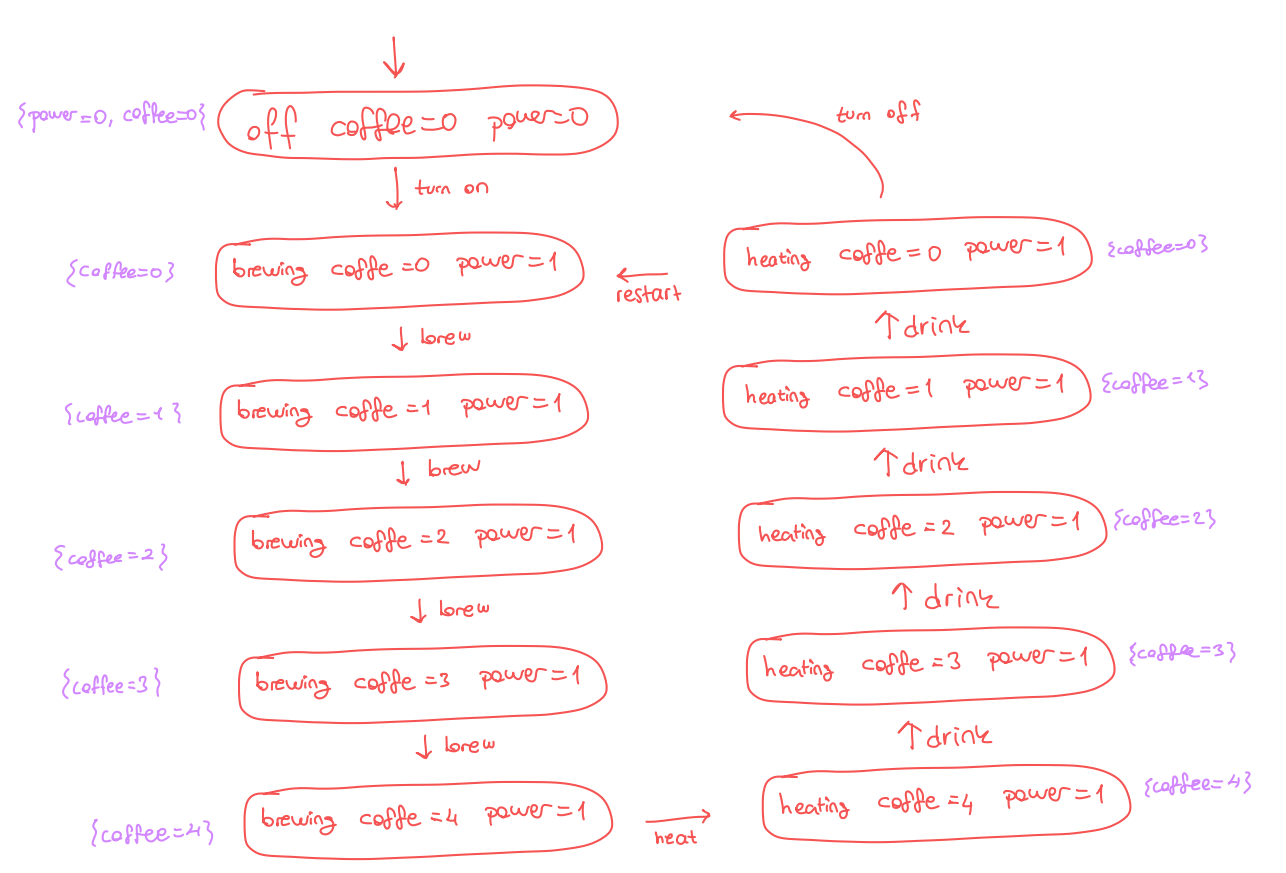
\includegraphics[width=5in]{images/2b.png}
        \caption{Transition system of coffee machine, with labels}
        \label{fig:2b}
    \end{figure}
\end{enumerate}

\newpage

\section*{Exercise 3: Executions, Paths and Traces}

\begin{enumerate}[(a)]
    \item{Some execution and execution fragment examples:} \\
    \texttt{Execution:} A sequence of consecutive transactions, starting from initial state, ending in a final state or in an infinite loop. \\
    \texttt{Execution Fragment:} Some part of an execution. \\
    \begin{enumerate}[•]
        \item {An execution fragment that is neither initial nor maximal}
        $$
            s_2 \xrightarrow{Y} s_3 \xrightarrow{Y} s_4
        $$
        \item  {An initial execution fragment that is not maximal}
        $$
            s_0 \xrightarrow{\alpha} s_1 \xrightarrow{\alpha} s_1
        $$
        \item  {A maximal execution fragment that is not initial}
        $$
            s_1 \xrightarrow{\alpha} s_1 \xrightarrow{\alpha} s_1 ...
        $$
        \item  {An initial and maximal execution fragment (i.e. an execution)}
        $$
            s_0 \xrightarrow{\alpha} s_1 \xrightarrow{\alpha} s_1 ...
        $$
    \end{enumerate}
    
    \item \textbf{How many executions does the transition system have?}\\
    Because of two loops next to each other, ($s_2$ on itself and the one between $s_2$ and $s_3$), there can be infinitely many execution combinations created. 
    \item \textbf{Provide a path of the transition system. How many are there in total?}\\
    There are infinitely many paths in the system. Here are some examples:
    $$ s_0, s_1, s_1, s_1 ...$$
    $$ s_0, s_2, s_2, s_2 ...$$
    $$ s_0, s_2, s_3, s_2, s_3...$$
    $$ s_0, s_2, s_2, s_3, s_2, s_2, s_3...$$
    \item \textbf{How many traces does the transition system have?}\\
    There are 2 traces of this system:
    $$ \emptyset, a, a, ... = \{\emptyset \} \{a\}^\omega $$
    $$ \emptyset, b, b, ... = \{\emptyset \} \{b\}^\omega $$
    \item \textbf{Bonus: Is it possible to have a transition system with infinitely many executions and finitely many paths?}\\
    Yes, it is possible.
    \begin{figure}[h] 
        \centering
        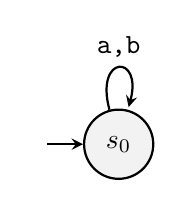
\begin{tikzpicture}
            \node[state, initial] (s0) {$s_0$};
            \draw (s0) edge[loop above] node {\tt a,b} (s0);
        \end{tikzpicture}
        \label{fig:bonus}
    \end{figure}
\end{enumerate}


\end{document}
